\documentclass[a4paper]{article}


% import packages
\usepackage{graphicx}  % for \includegraphics with jpg,png,...
\usepackage[english,ngerman]{babel}  % ngerman: Neue Rechtschreibung
\usepackage{url}
\usepackage[dvipsnames]{xcolor}  % for \color
\usepackage{listings}  % source code support
\usepackage[utf8]{inputenc}
\usepackage{textcomp}  % support for symbols like €
\usepackage{lmodern}  % improve font
\usepackage{float}  % allow H option in \begin{figure}[H]
\usepackage{caption}


% configure packages
\setlength{\columnsep}{8mm}

\definecolor{codebg}{HTML}{eff0f1}
\lstset{
    backgroundcolor=\color{codebg},
    breaklines=true,
    tabsize=2,
    basicstyle=\small\ttfamily\bfseries,
    postbreak=\kern-5ex\mbox{\textcolor{gray}{$\hookrightarrow$}\space},
    numbers=left,
    numberstyle=\color{gray},
    showspaces=false,
    showstringspaces=false,
    tabsize=1,
    frame=single,
    rulecolor=\color{white},
    xleftmargin=3pt,
    xrightmargin=3pt,
}
% from https://github.com/cansik/kotlin-latex-listing
\lstdefinelanguage{Kotlin}{
    comment=[l]{//},
    commentstyle={\color{gray}\ttfamily},
    emph={delegate, filter, first, firstOrNull, forEach, lazy, map, mapNotNull, println, return@},
    emphstyle={\color{OrangeRed}},
    identifierstyle=\color{black},
    keywords={abstract, actual, as, as?, break, by, class, companion, continue, data, do, dynamic, else, enum, expect, false, final, for, fun, get, if, import, in, interface, internal, is, null, object, override, package, private, public, return, set, super, suspend, this, throw, true, try, typealias, val, var, vararg, when, where, while},
    keywordstyle={\color{NavyBlue}\bfseries},
    morecomment=[s]{/*}{*/},
    morestring=[b]",
    morestring=[s]{"""*}{*"""},
    ndkeywords={@Deprecated, @JvmField, @JvmName, @JvmOverloads, @JvmStatic, @JvmSynthetic, Array, Byte, Double, Float, Int, Integer, Iterable, Long, Runnable, Short, String},
    ndkeywordstyle={\color{BurntOrange}\bfseries},
    sensitive=true,
    stringstyle={\color{ForestGreen}\ttfamily},
}

\setlength{\parindent}{0cm}  % remove paragraph indentation
\setlength{\intextsep}{8pt}  % set space between two float objects

\raggedbottom  % move spacing produced by figures to the bottom of the page


\begin{document}

\title{\textbf{stock-simulator}}
\author{
    Jan Müller\\
    Jonas Thelemann\\
    Juri Lozowoj\\
    Lucas Held
}
\date{27. März 2020}
\maketitle

\pagebreak
\tableofcontents
\pagebreak

\begin{lstlisting}[caption={example kotlin code}, captionpos=b, label={lst:example}, language=Kotlin]
private suspend fun StockbrotQuote.executeSellOrder(quote: Quote) {
    val depotQuote = accountRepository.depotQuoteBySymbol(id) ?: return
    if (quote.latestPrice >= minimumSellPrice) {
        val amount = depotQuote.amount
        Timber.i("Bot is selling $amount for ${quote.latestPrice}")
        accountRepository.sell(quote, amount)
    }
}
\end{lstlisting}

\begin{figure}[H]
    \centering
    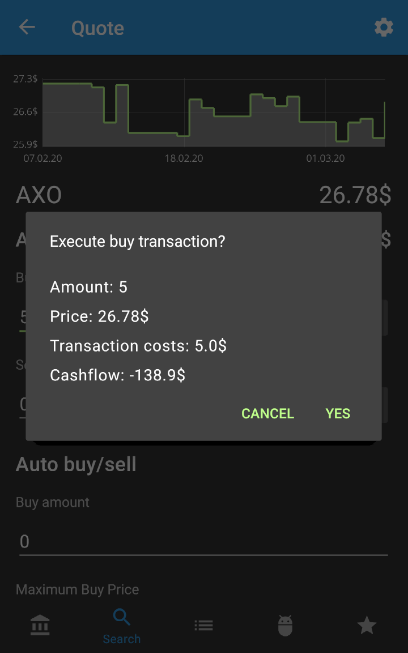
\includegraphics[height=10cm,keepaspectratio]{./images/quote_buy_confirmation_dialog.png}
    \caption{example image}
    \label{fig:example}
\end{figure}

\pagebreak


\section{Einleitung}
% Gute Einleitung ins Thema (was war die Aufgabe, etc.)
Aufgabe der Veranstaltung "`Code-Camp Context-Awareness 1"' war die Entwickelung eines Börsensimulator Spiels für Android Smartphones. Dabei stellte das Verwenden von echten Aktienkursen, mit aktuellen Daten, eine wichtige Anforderung an das Spiel dar. Diese Daten sollten als Basis für alle weiteren Funktionen dienen. Mithilfe des zur Verfügung stehenden Spielgeldes soll der Benutzer die Möglichkeit haben, Aktien oder Kryptowährungen zu kaufen. Um das Kaufen von bestimmten Aktien und Kryptowährungen zu ermöglichen, wurde eine Suchfunktion gefordert, welche die verfügbaren Elemente filtert und anzeigt. Um das Budget immer im Blick zu behalten, muss es Depotübersicht, sowie eine Anzeige für den aktuellen Kontostand und dessen Verlauf geben. Eine Historie soll die Käufe und Verkäufe in der Vergangenheit darstellen. Als Darstellungsform der Kurse und des Kontoverlaufs sind Graphen zu wählen. Wie auf gängigen Tradingplatformen soll auch der Simulator mit jedem Kauf- oder Verkauf Transaktionskosten berechnen. Ein Bot soll das Traden übernehmen, falls dies vom Benutzer gewünscht wird. Entsprechende Zielwerte sollen für jede Aktie oder Kryptowährung anpassbar sein. Damit der Benutzer die Möglichkeit hat, das Spiel neu zu beginnen, muss die Anwendung eine Option bieten, den Spielstand zurückzusetzen. Zusätzlich zu den bisher genannten Hauptfeatures, wird mindestens ein Zusatzfeature gefordert, welches eine nützliche Erweiterung für die Anwendung darstellt. Ziel des Spiels ist es, das Startkapital im Laufe der Zeit möglichst stark zu vermehren.


\section{Technische Details}
TODO


\subsection{Architektur}
% App Architektur (Welches Pattern habt ihr benutzt? MVVM? Livedata?) Was ist das und warum ist das cool?
% Schwierigkeiten und wie ihr sie gelöst habt
TODO


\subsection{APIs}
TODO


\subsubsection{IEX Cloud}
% https://iexcloud.io/
TODO


\subsubsection{CoinGecko}
% https://www.coingecko.com/
TODO


\subsection{Bibliotheken}
TODO


\subsubsection{Android Jetpack}
% https://developer.android.com/jetpack/
TODO


\subsubsection{Moshi}
% https://github.com/square/moshi
TODO


\subsection{Room}
% https://developer.android.com/jetpack/androidx/releases/room
TODO


\subsubsection{Retrofit}
% https://github.com/square/retrofit
TODO


\section{Funktionalität}
% Welche Features habt ihr gebaut?
% Welche Screens habt ihr gebaut?
% Warum sehen die Screens so aus? (warum ist button X an Position Y) / was habt ihr euch dabei gedacht?
TODO


\section{Teamwork}
TODO


\section{Zusammenfassung}
TODO


\section{Fazit}
TODO


\section{Ausblick}
% was kann man noch machen, was habt ihr nicht geschafft,..
TODO


\end{document}
